% !TeX root = ../../main.tex
\newpage

\newpage
\section{Zbiory danych}

Do przeprowadzenia eksperymentów użyto dwóch zbiorów danych, w skład których wchodzą między innymi zdjęcia otrzymane od firmy ``BLUE''.
Jeden zbiór, zwany dalej zbiorem \textit{high} pochodzi z kamer ustawianych ponad kortem.
Drugi zbiór, zwany dalej zbiorem \textit{low}, pochodzi z kamer sytuowanych na podłodze, tuż przy liniach kortu.


\begin{figure}[!htb]
  \minipage{0.45\textwidth}
    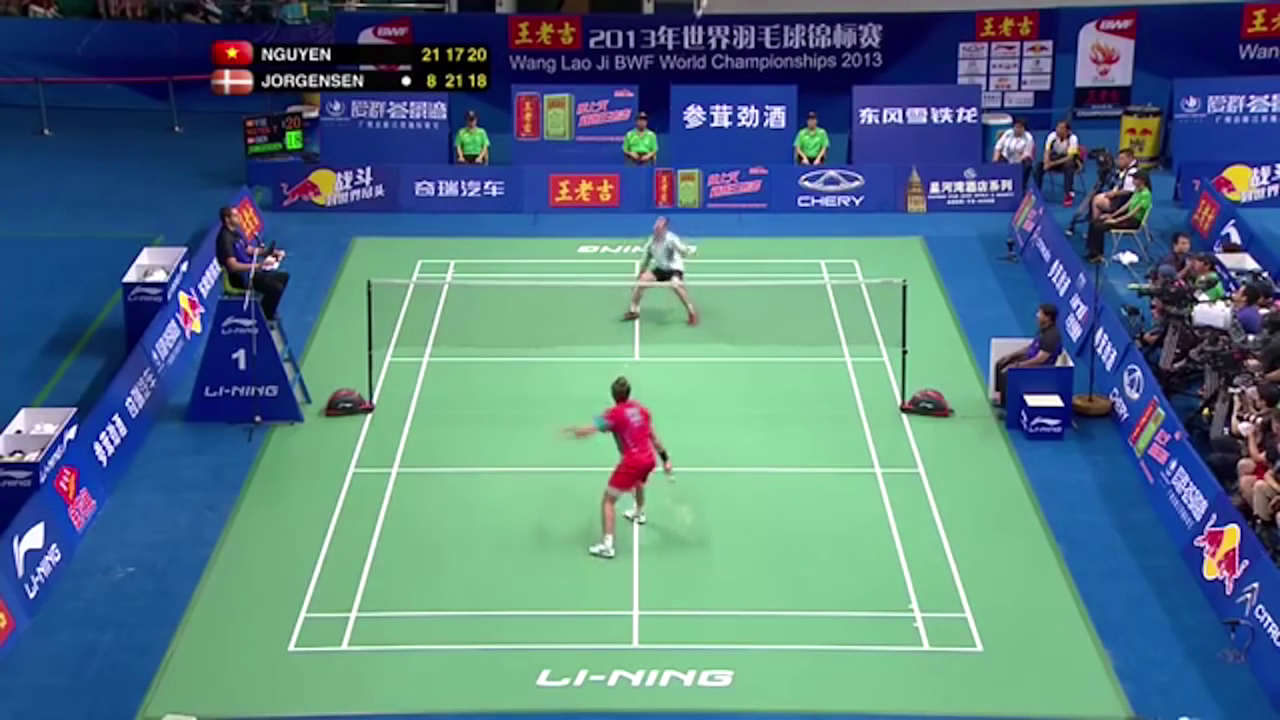
\includegraphics[width=\linewidth]{../../badminton/datasets/high/split/test_court2-00002.png}
    \caption{Przykładowy obraz ze zbioru danych \textit{high}}
  \endminipage\hfill
  \minipage{0.45\textwidth}
    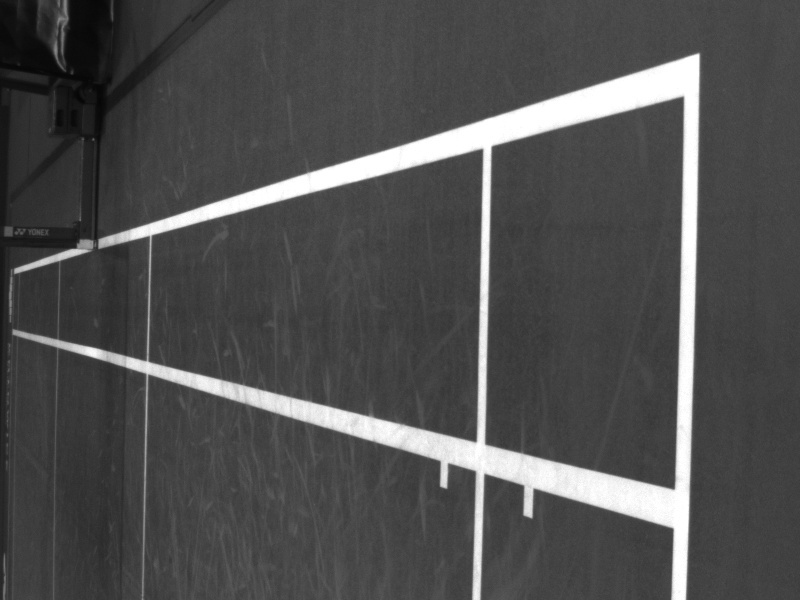
\includegraphics[width=\linewidth]{../../badminton/datasets/low/split/1564909032792410075.jpg}
    \caption{Przykładowy obraz ze zbioru danych \textit{low}}
  \endminipage\hfill
\end{figure}

Zbiór danych \textit{high} składa się z obrazów o różnych rozmiarach, i pochodzących z różnych źródeł.
Zbiór \textit{low} zawiera obrazy pozyskane wyłącznie od firmy ``BLUE'', o rozdzielczości 896x640 pikseli.

\begin{table}[!h]
	\centering
	\caption{Liczność zbiorów danych}
	\vspace{6pt}
	{\footnotesize
		\begin{tabular}{|c|c|c|c|}
			\hline \textbackslash & Liczność \\
      \hline Zbiór \textit{high} & 97 \\
      \hline Zbiór \textit{low} & 207 \\
      \hline
		\end{tabular}
	}
	\vspace{0pt}
\end{table}

\newpage
\subsection{Podział na podzbiory treningowe, walidacyjne i testowe}
W tym podrozdziale omówiona zostanie strategia podziału zbiorów danych na podzbiory treningowe, walidacyjne i testowe.
Ze względu na stosunkowo małą liczność zbiorów danych, podzbiór testowy został ograniczony do dwóch obrazów.
Pozostałe obrazy, wchodzące w skład podzbiorów treningowych i walidacyjnych, zostały rozdzielone po przeprowadzeniu eksperymentów, tak aby wybrany podział dawał możliwe najlepsze rezultaty.
Rozważono następujące podziały:

\begin{table}[!h]
	\centering
	\caption{Liczba obrazów w podziale na poszczególne podzbiory}
	\vspace{6pt}
	{\footnotesize
		\begin{tabular}{|c|c|c|c|}
			\hline \textbackslash & Podzbiór treningowy & Podzbiór walidacyjny & Podzbiór testowy \\
      \hline Zbiór \textit{high} & 92 (94.85\%) & 5 (5.15\%) & 2 (2.06\%) \\
      \hline Zbiór \textit{high} & 87 (89.69\%) & 10 (10.31\%) & 2 (2.06\%) \\
      \hline Zbiór \textit{high} & 73 (75.26\%) & 24 (24.74\%) & 2 (2.06\%) \\
      \hline Zbiór \textit{high} & 49 (50.52\%) & 48 (49.48\%) & 2 (2.06\%) \\
      \hline Zbiór \textit{low} & 197 (95.17\%) & 10 (4.83\%) & 2 (0.97\%) \\
      \hline Zbiór \textit{low} & 186 (89.86\%) & 21 (10.14\%) & 2 (0.97\%) \\
      \hline Zbiór \textit{low} & 155 (74.88\%) & 52 (25.12\%) & 2 (0.97\%) \\
      \hline Zbiór \textit{low} & 104 (50.24\%) & 103 (49.76\%) & 2 (0.97\%) \\
      \hline
		\end{tabular}
	}
	\vspace{0pt}
\end{table}


W kolejnych podrozdziałach przedstawiono rezultaty sieci trenowanej z użyciem podzbiorów podzielonych według poszczególnych podziałów.

\TODO{TP, TN itp nie mają sensu dla high, tylko dla low (bo obrazki tej samej rozdzielczości)}

\subimport{}{highsplita}
\subimport{}{highsplitb}
\subimport{}{highsplitc}
\subimport{}{highsplitd}
\subimport{}{lowsplita}
\subimport{}{lowsplitb}
\subimport{}{lowsplitc}
\subimport{}{lowsplitd}
\subimport{}{summary}

\newpage
Zbiory podzielone są na podzbiory treningowe, walidacyjne oraz testowe w następujący sposób (wraz z porównaniem ze zbiorem COCO \cite{coco}):

\begin{table}[!h]
	\centering
	\caption{Liczba obrazów w podziale na poszczególne podzbiory}
	\vspace{6pt}
	{\footnotesize
		\begin{tabular}{|c|c|c|c|}
			\hline \textbackslash & Podzbiór treningowy & Podzbiór walidacyjny & Podzbiór testowy \\
      \hline Zbiór \textit{low} & 156 & 51 & 2 \\
      \hline Zbiór \textit{high} & 134 & 7 & 2 \\
      \hline Zbiór COCO & ok. 118000 & ok. 5000 & ok. 41000 \\
      \hline
		\end{tabular}
	}
	\vspace{0pt}
\end{table}

